% =============================================================================
% FIGURES — TikZ/PGFPlots for Chapter 4
% =============================================================================

% Color palette
\definecolor{gcrgold}{RGB}{218,165,32}
\definecolor{dcagreen}{RGB}{34,139,34}
\definecolor{dcablue}{RGB}{70,130,180}

% =============================================================================
% Figure 1: Path Statistics Before/After Filtering (Grouped Bar)
% =============================================================================
\begin{figure}[htbp]
  \centering
  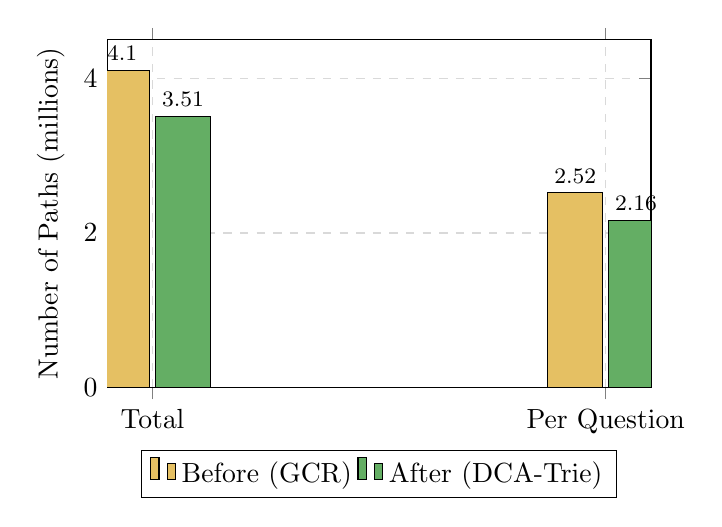
\begin{tikzpicture}
    \begin{axis}[
      ybar,
      bar width=20pt,
      width=0.7\textwidth,
      height=6cm,
      ylabel={Number of Paths (millions)},
      symbolic x coords={Total, Per Question},
      xtick=data,
      ymin=0,
      ymax=4.5,
      legend style={at={(0.5,-0.18)}, anchor=north, legend columns=-1},
      nodes near coords,
      every node near coord/.append style={font=\footnotesize},
      grid=major,
      grid style={dashed, gray!30},
    ]
    \addplot[fill=gcrgold!70] coordinates {(Total, 4.10) (Per Question, 2.52)};
    \addplot[fill=dcagreen!70] coordinates {(Total, 3.51) (Per Question, 2.16)};
    \legend{Before (GCR), After (DCA-Trie)}
    \end{axis}
  \end{tikzpicture}
  \caption{Path Statistics (4.10M → 3.51M)}
  \label{fig:path_stats}
\end{figure}

% =============================================================================
% Figure 2: Gate Decomposition (Grouped Bar)
% =============================================================================
\begin{figure}[htbp]
  \centering
  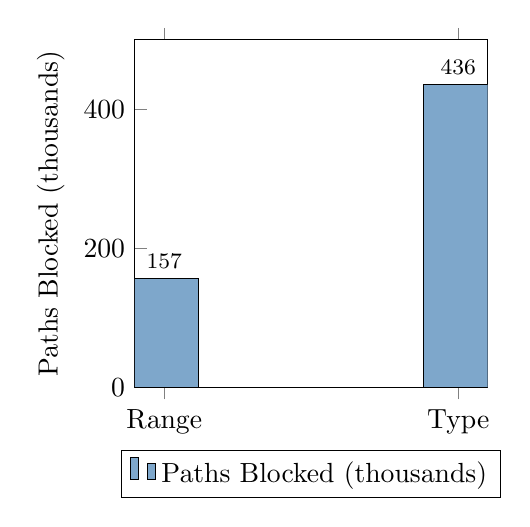
\begin{tikzpicture}
    \begin{axis}[
      ybar,
      bar width=25pt,
      width=0.5\textwidth,
      height=6cm,
      ylabel={Paths Blocked (thousands)},
      symbolic x coords={Range, Type},
      xtick=data,
      ymin=0,
      ymax=500,
      legend style={at={(0.5,-0.18)}, anchor=north, legend columns=-1},
      nodes near coords,
      every node near coord/.append style={font=\footnotesize},
    ]
    \addplot[fill=dcablue!70] coordinates {(Range, 157) (Type, 436)};
    \legend{Paths Blocked (thousands)}
    \end{axis}
  \end{tikzpicture}
  \caption{Gate Decomposition (Range: 3.8\%, Type: 10.6\%)}
  \label{fig:gate_decomp}
\end{figure}

% =============================================================================
% Figure 3: FNR by Gate (Horizontal Bar with Threshold)
% =============================================================================
\begin{figure}[htbp]
  \centering
  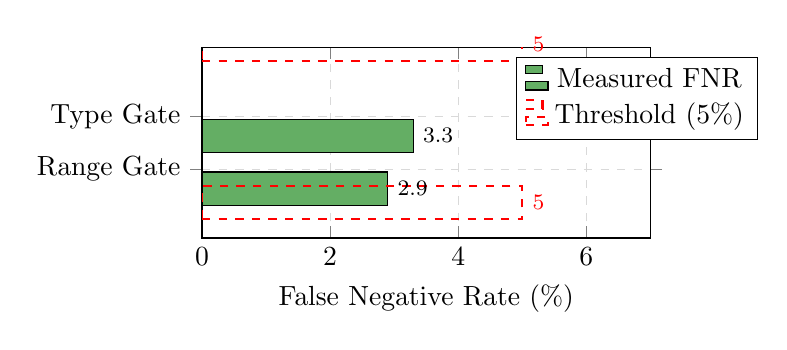
\begin{tikzpicture}
    \begin{axis}[
      xbar,
      bar width=12pt,
      width=0.6\textwidth,
      height=4cm,
      xlabel={False Negative Rate (\%)},
      ytick={1,2},
      yticklabels={Range Gate, Type Gate},
      xmin=0,
      xmax=7,
      legend style={at={(0.7,0.95)}, anchor=north west},
      nodes near coords,
      every node near coord/.append style={font=\footnotesize},
      grid=major,
      grid style={dashed, gray!30},
    ]
    \addplot[fill=dcagreen!70] coordinates {(2.9, 1) (3.3, 2)};
    \addplot[red, dashed, thick] coordinates {(5, 0) (5, 3)};
    \legend{Measured FNR, Threshold (5\%)}
    \end{axis}
  \end{tikzpicture}
  \caption{False Negative Rates (<5\%)}
  \label{fig:fnr}
\end{figure}

% =============================================================================
% Figure 4: Hits@1 and F1 Comparison (Grouped Bar)
% =============================================================================
\begin{figure}[htbp]
  \centering
  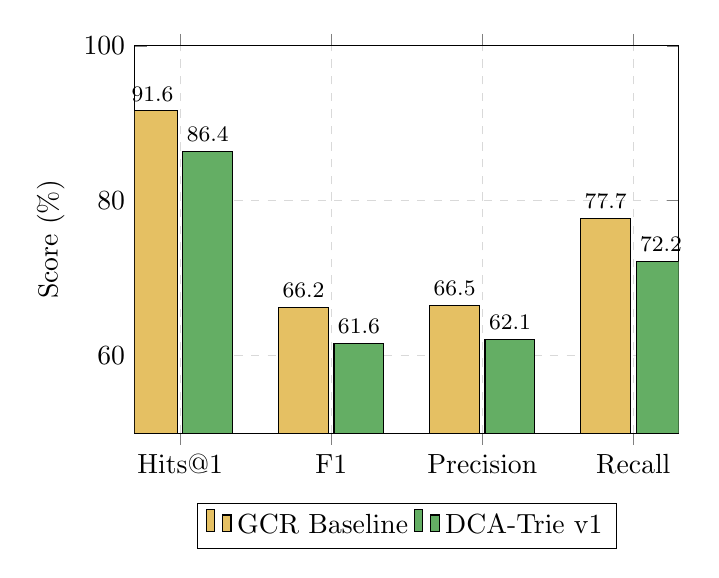
\begin{tikzpicture}
    \begin{axis}[
      ybar,
      bar width=18pt,
      width=0.7\textwidth,
      height=6.5cm,
      ylabel={Score (\%)},
      symbolic x coords={Hits@1, F1, Precision, Recall},
      xtick=data,
      ymin=50,
      ymax=100,
      legend style={at={(0.5,-0.18)}, anchor=north, legend columns=-1},
      nodes near coords,
      every node near coord/.append style={font=\footnotesize},
      grid=major,
      grid style={dashed, gray!30},
    ]
    \addplot[fill=gcrgold!70] coordinates {(Hits@1, 91.6) (F1, 66.2) (Precision, 66.5) (Recall, 77.7)};
    \addplot[fill=dcagreen!70] coordinates {(Hits@1, 86.4) (F1, 61.6) (Precision, 62.1) (Recall, 72.2)};
    \legend{GCR Baseline, DCA-Trie v1}
    \end{axis}
  \end{tikzpicture}
  \caption{WebQSP Performance}
  \label{fig:main_results}
\end{figure}

% =============================================================================
% Figure 5: Execution Time Comparison (Grouped Bar)
% =============================================================================
\begin{figure}[htbp]
  \centering
  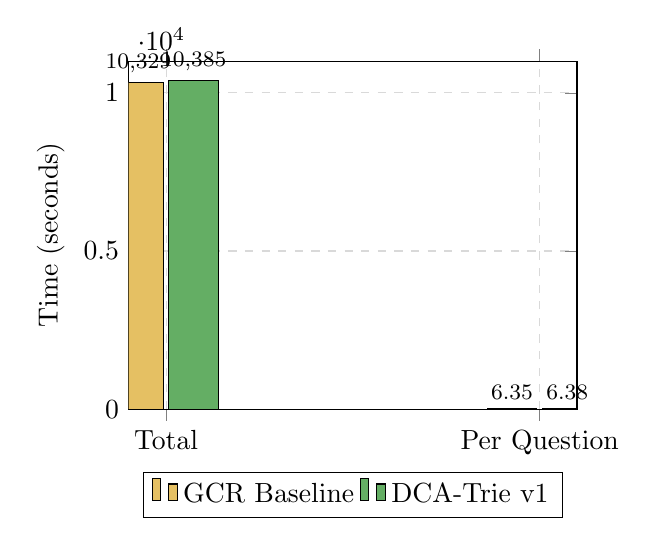
\begin{tikzpicture}
    \begin{axis}[
      ybar,
      bar width=18pt,
      width=0.6\textwidth,
      height=6cm,
      ylabel={Time (seconds)},
      symbolic x coords={Total, Per Question},
      xtick=data,
      ymin=0,
      ymax=11000,
      legend style={at={(0.5,-0.18)}, anchor=north, legend columns=-1},
      nodes near coords,
      every node near coord/.append style={font=\footnotesize},
      grid=major,
      grid style={dashed, gray!30},
    ]
    \addplot[fill=gcrgold!70] coordinates {(Total, 10329) (Per Question, 6.35)};
    \addplot[fill=dcagreen!70] coordinates {(Total, 10385) (Per Question, 6.38)};
    \legend{GCR Baseline, DCA-Trie v1}
    \end{axis}
  \end{tikzpicture}
  \caption{Execution Time Comparison}
  \label{fig:timing}
\end{figure}

% =============================================================================
% Figure 6: Non-Monotone Relationship (Conceptual Scatter)
% =============================================================================
\begin{figure}[htbp]
  \centering
  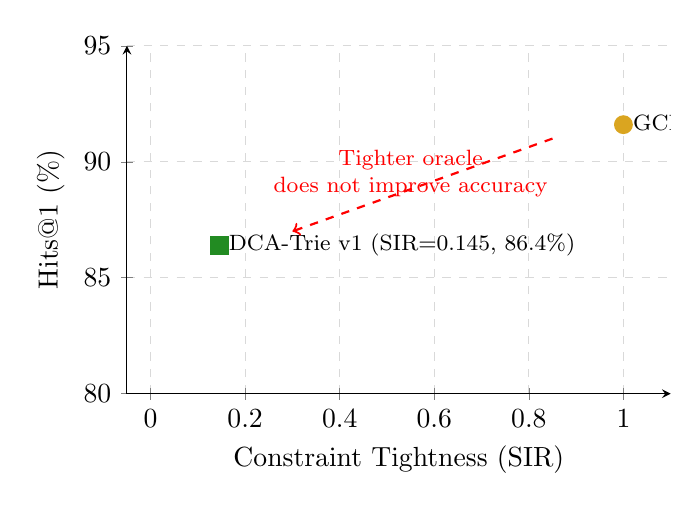
\begin{tikzpicture}
    \begin{axis}[
      width=0.7\textwidth,
      height=6cm,
      xlabel={Constraint Tightness (SIR)},
      ylabel={Hits@1 (\%)},
      xmin=-0.05,
      xmax=1.1,
      ymin=80,
      ymax=95,
      grid=major,
      grid style={dashed, gray!30},
      axis lines=left,
    ]
    \addplot[mark=*, mark size=3pt, gcrgold, thick] coordinates {(1.0, 91.6)};
    \node[right, font=\footnotesize] at (axis cs:1.0, 91.6) {GCR (SIR=1.0, 91.6\%)};
    \addplot[mark=square*, mark size=3pt, dcagreen, thick] coordinates {(0.145, 86.4)};
    \node[right, font=\footnotesize] at (axis cs:0.145, 86.4) {DCA-Trie v1 (SIR=0.145, 86.4\%)};
    \draw[->, thick, red, dashed] (axis cs:0.85, 91.0) -- (axis cs:0.3, 87.0);
    \node[red, font=\footnotesize, align=center] at (axis cs:0.55, 89.5) {Tighter oracle\\does not improve accuracy};
    \end{axis}
  \end{tikzpicture}
  \caption{Non-Monotone Relationship}
  \label{fig:non_monotone}
\end{figure}
